\chapter{Metodology}
\label{chap:Metodology}

This chapter is about describing the metodology and developments to achieve the project goals. 
The python routine which this project is about was developed by the previous student that worked on it.\cite{Monica}
The works therefore presented here are a continuation and optimization of the routine to make it more precise and applicable to both industrial and research approaches.

About the activities made to reach our goals, it highlights the following:

- Integrate high speed camera and liquid pump to the peripherals connected to the software.

- Develop of a control model to automatic stabilize the electrospraying mode.

- Remodel the software to support threads in order to separate each subsystem and exchange data beetween them with use of queues data structures.

- Reduce the data collected size and optimize the saving to a real time streamming.

- Develop new automatic experiment routines such as mapping and control routines.

- Reestructure the setup file and the algorithm usability in order to make it more intuitive.

- Integration with many computer architectures to be able to run in a portable computer such as a \emph{Raspberry Pi}.
    
    \begin{figure}[H]
        \centering
        \resizebox{150mm}{!}{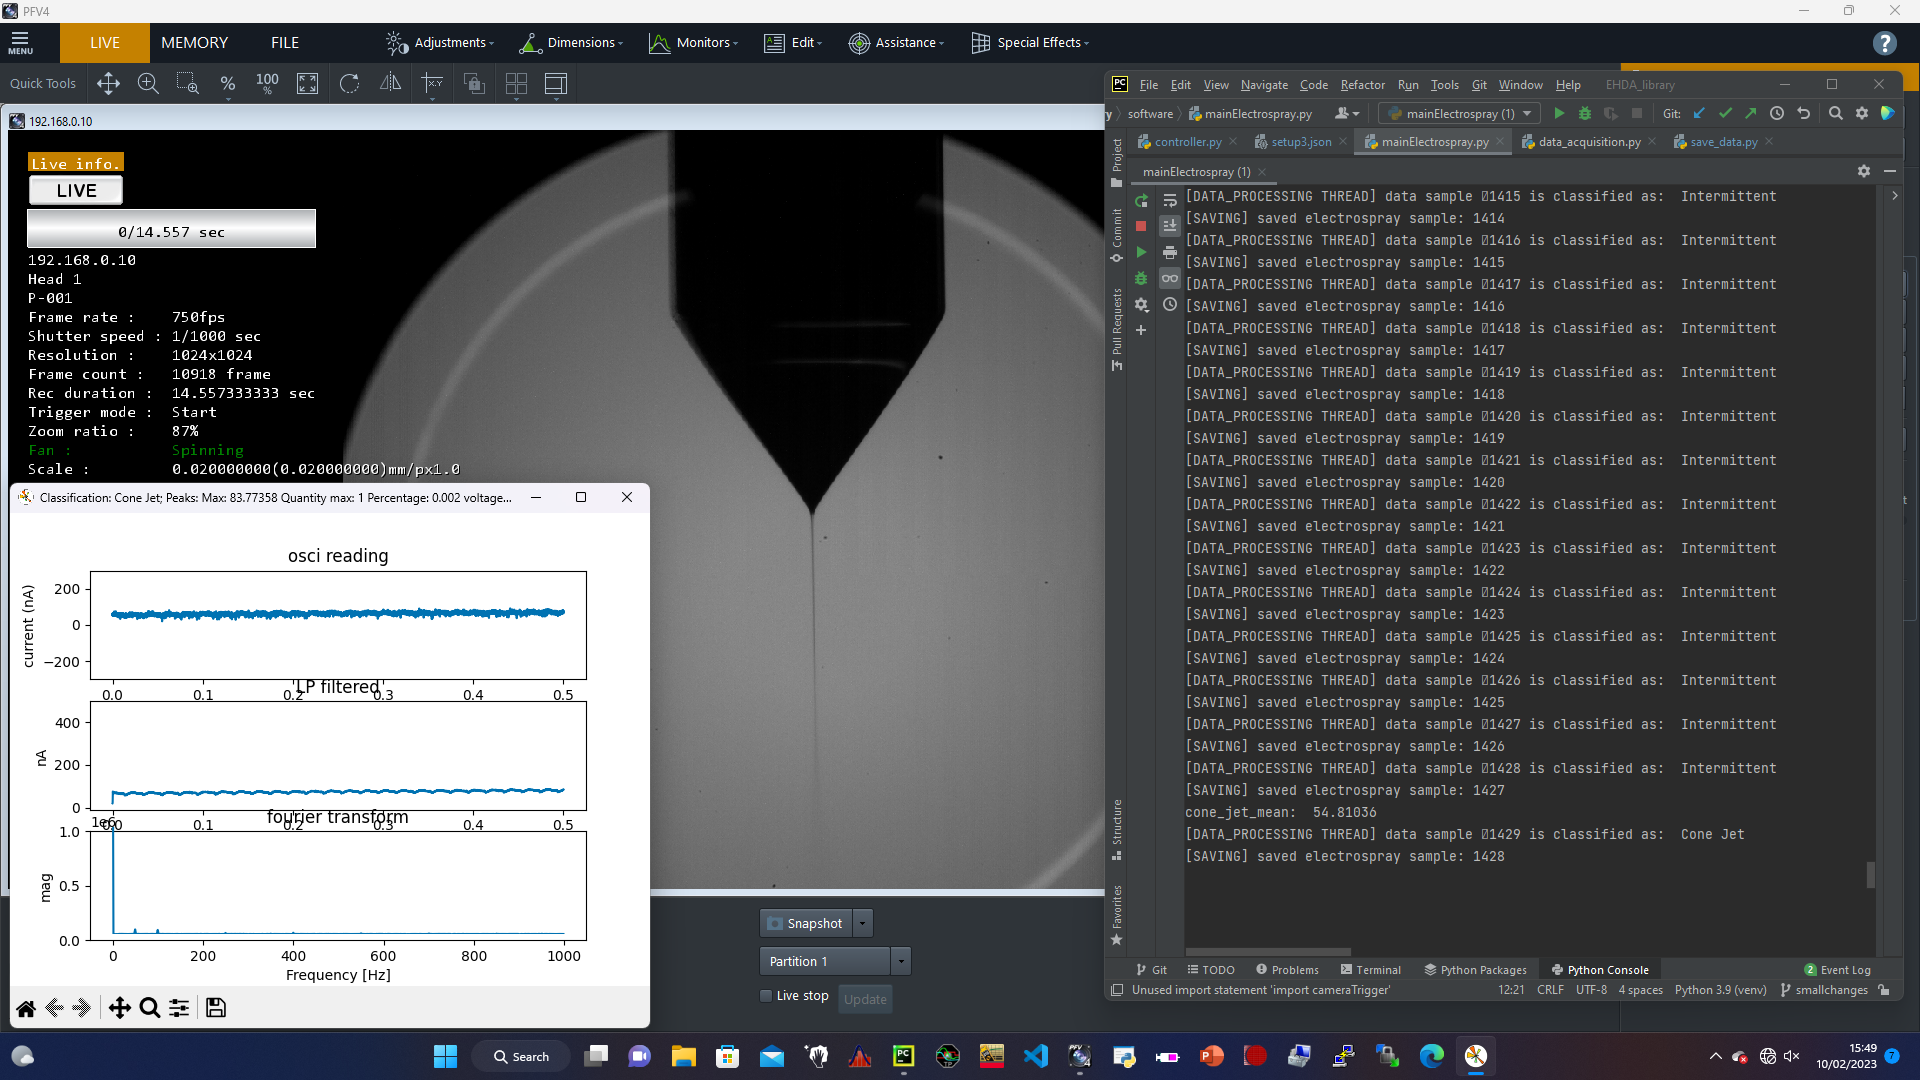
\includegraphics{Figuras/report4/experiment_print1.png}}
        \caption{EHDA automation system setup}
        \label{fig:metodology_example1}
    \end{figure}

\section{System Model}
\label{sec:control_model}

ilustramos o processo com a Figura \ref{fig:control_model_fig}. 

\begin{figure}[H]
  \centering
  \resizebox{150mm}{!}{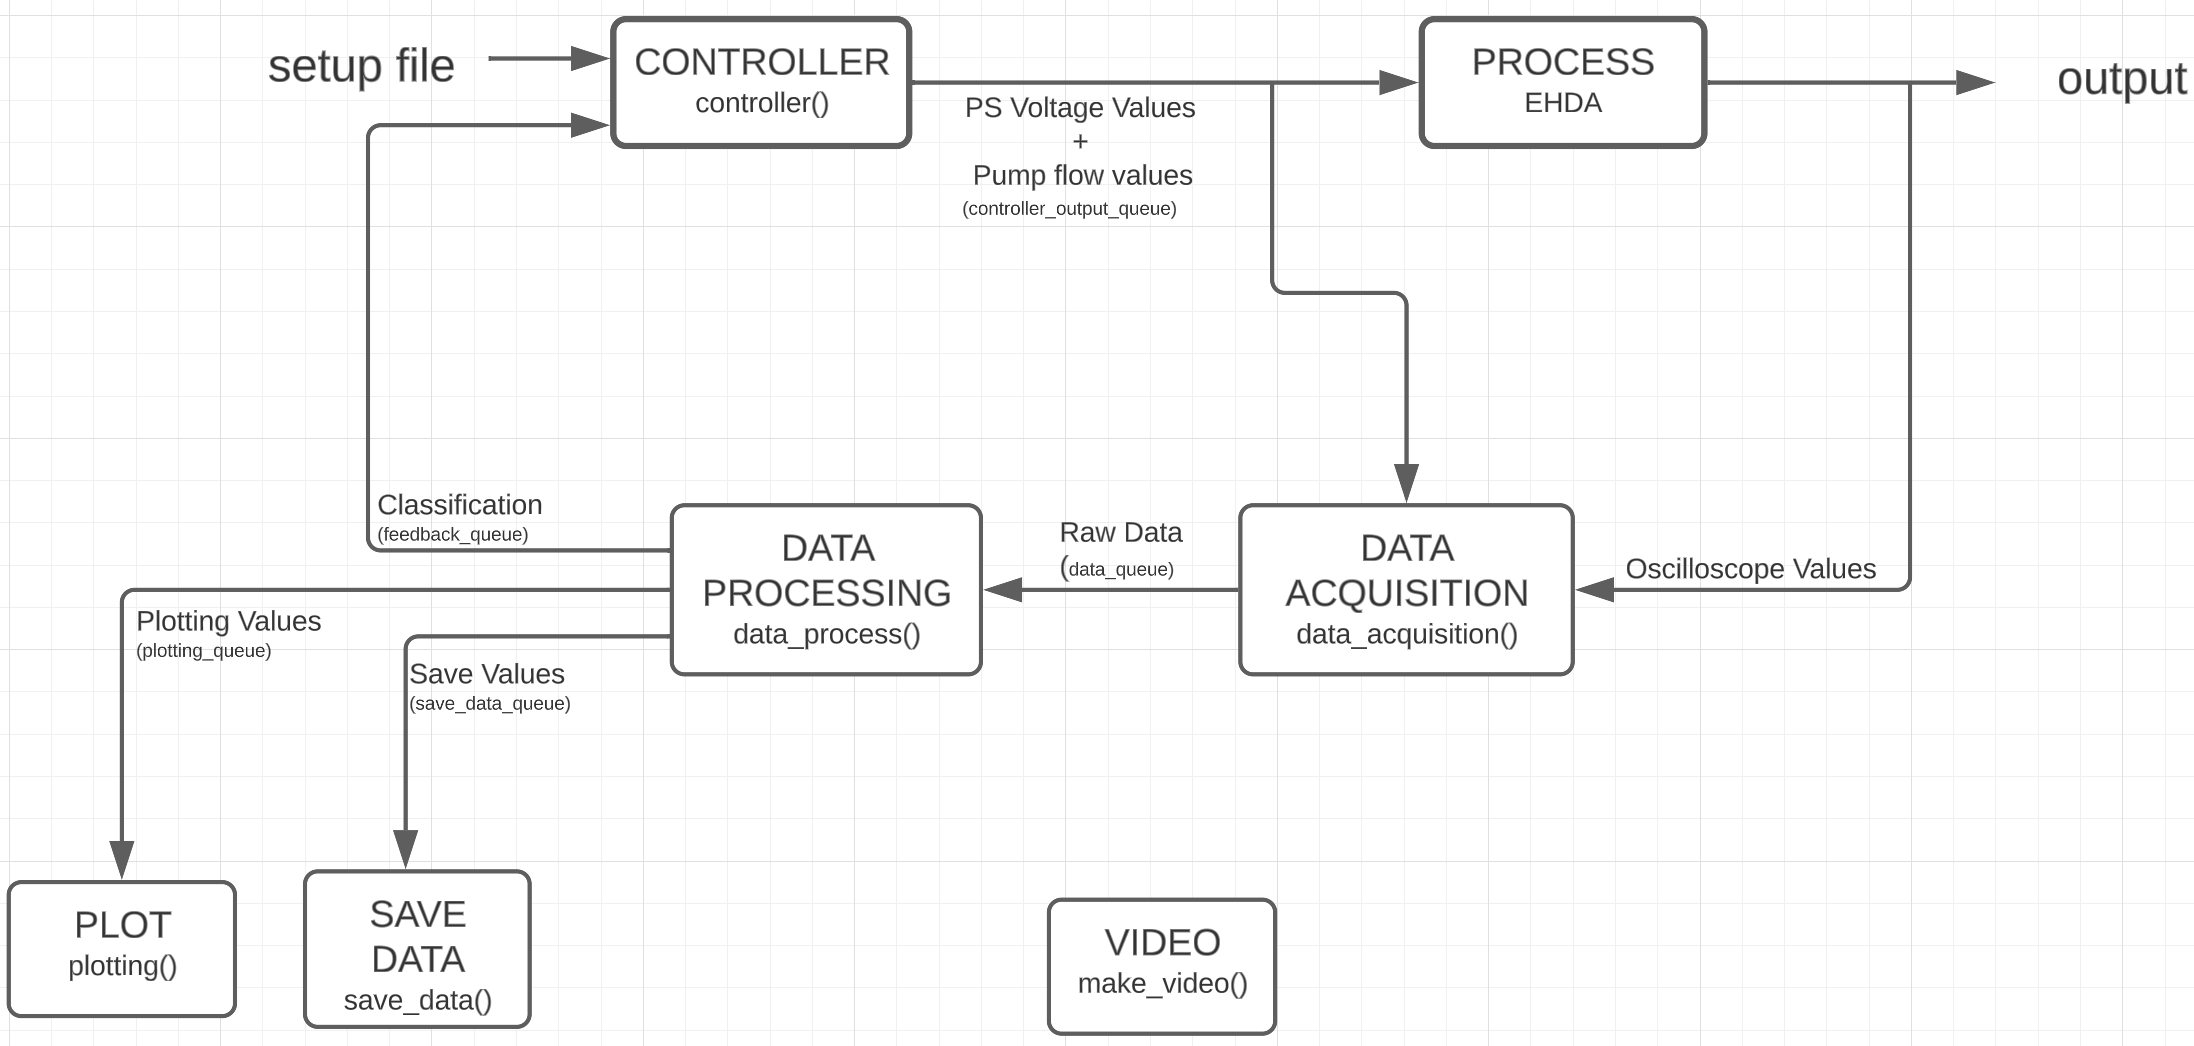
\includegraphics{Figuras/control_loop.png}}
  \caption{EHDA automation system setup}
  \label{fig:control_model_fig}
\end{figure}

\subsection{Threading and Queues}
\label{subsec:concurrency}

    In order to implement this system model to the software and explore parallel processing each system in the
    model was developed as a separate Thread.
    For cuncurrency on flux of data beetween threads was used queues structures.
    A queue is an abstract data type that holds an ordered, linear sequence of items. You can describe it as a first in, first out (FIFO) structure.

    
    \subsection{Controller Thread}

        It is responsible of sending the power supply set voltage values and the syringe pump the flow rate set values according to the sequence selected.
        Also responsible of sending the finish event command that end the routine and trigger the threads to close their routines.
        As input we have the setup config file and the \emph{feedback\_queue}. As output we have the values in the emph{controller\_output\_queue()}.

    \subsection{Data Acquisition Thread}

        It is responsible for reading the current data from the oscilloscope, humidity and temperature data from the DHT11 sensor, voltage from the powersupply, flowrate from the pump and concatenate into one sample data.
        As output we have the values in the emph{data\_queue()}.

    \subsection{Data Processing Thread}

        It is responsible for calculating the statistical values from the raw data and classify it in the respective spray mode for that sample.
        As output we have the values in the emph{save\_data\_queue()}, emph{plotting\_queue()} and emph{feedback\_queue()}.
    
        \subsection{Save Data Thread}

        After the processing the data is saved in real time in a json file using \emph{jsonstreams} library to save one sample structure at a time.

        With the new streamming model of saving a new structure of the collected data were created.
        Instead of having all data measurements values and after all data processing values we now are saving for each sample the measurements and processing values.
        The structure of the 
    
        \begin{figure}[H]
            \center
            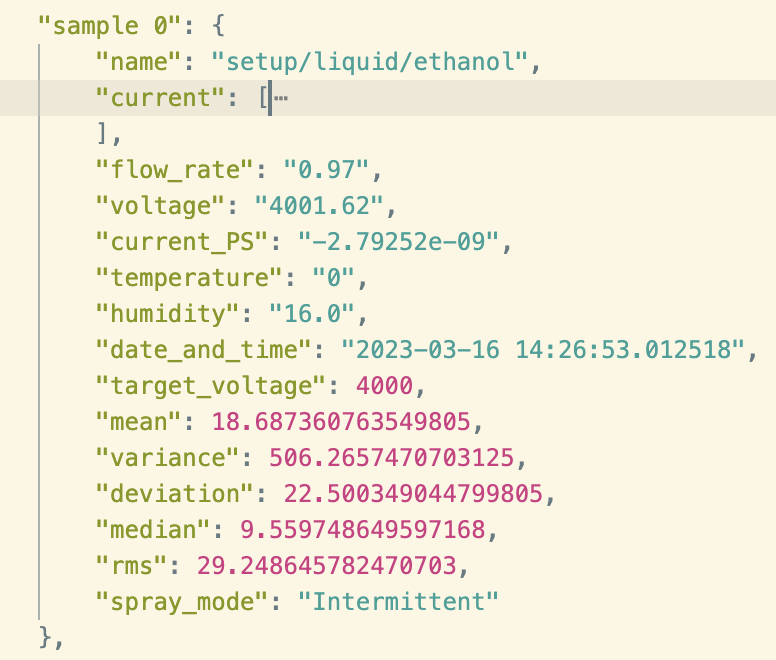
\includegraphics[width=10cm]{Figuras/19:03/new_sample.png}
            \caption{Output data json structure}
        \end{figure}
    
        To work with this data I'm using pandas Dataframe.
        With the command:
        
        pandas.read\_json('PATH', orient='index').
    
        The json file is good to store the data and to read the file. But as it is getting a lot of data working with pandas Dataframe is being way faster. Also saving the dataframe in a compressed
        type of file called feather is much faster to work with the data.
    
    \subsection{Video Thread}

        Normally deactivated, that thread is responsible for triggering the camera in case we want to save a video of that sample.
    
    \subsection{Plot}

        The only running function that is not a thread because of the plotting library \emph{matplotlib} incompatibilites of running outside of the main function. 
        It is responsible of plotting in real time the current sample acquired and it respective fast fourier transform to evaluate the sample frequency spectrum.
    
    
    - plotting data queue


\section{Classification}
\label{sec:section_classification}

The classification is a key step in our routine. For being able to be used in multipurpose applications our classification routine must be able to run in real-time. Which means it must be fast and automatic classification.
Our goal is to improve and apply in our routine different approachs of non-visual spraying classification using the current data collected from the system.

\subsection{Statistical Analisys}

 According to Sjaaks\cite{Sjaaks}, evaluating the current data flowing through the nozzle to the plate can give us valuable information about the spraying behaviour.
 Together with the current characteristics, visual observations and results from literature it was investigated whether generic trends are present that can be related to the actual spraying modes.
 It was concluded that factors like geometry, polarity, material properties and occurring discharges are reflected in the system current.
In this work, the author also exposed some signal characteristics that can be used to classify the actual spraying mode with a sample of measured current using both time domain and frequency domain analysis.

From those analysis we are appliying in our automatic classification system the relative standard deviation. Which is refered as the sample standart deviation divided by the sample mean values.

\begin{figure}[H]
    \centering
    \resizebox{50mm}{!}{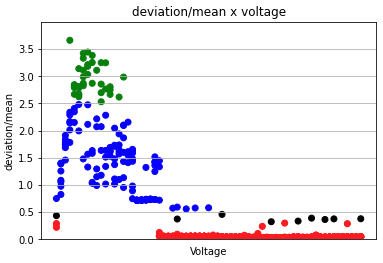
\includegraphics{Figuras/report2/data3_sjaaksgraph2.png}}
    \caption{EHDA automation system setup}
    \label{fig:sjaaks_statistical_class}
\end{figure}

 
 through statistical analysis in the signal such as mean value and standart deviation.
 Our classification by statistical analysis was implemented in the automation library made by the previous student \cite{Monica}.

 Each current sample is 0.5s of current data in 10kHz sampling frequency.
 By the processing thread we take this sample and evaluate the followings statistical values.
        
        - Sjaak Classification -> Classifies Dripping, Intermittent and Cone Jet
        
        - Monica Classification -> Classifies Corona Sparks

        - João Classification -> Classifies Multi Jet

	The algorithm implemented works in the following way:
	\begin{algorithm}
        \caption{Statistical Classification}\label{alg:statistical_class}
        \begin{algorithmic}
        \Function{statistical\_classification}{$sample$} 

            \State $spray\_mode \gets "Undefined"$;
            \State $mean \gets sample.mean$; 
            \State $std\_deviation \gets sample.std\_deviation$;
            \State $median \gets sample.median$;
            
            \If{ $mean / std\_deviation$ > 2.5}
                \Comment{Sjaak classification \cite{Sjaaks}} 
                \State $spray\_mode \gets "Dripping"$;
            \ElsIf{$ 2.5 < mean / std\_deviation < 2.5 \And mean / std\_deviation > 0.3 $}
                \State $spray\_ mode \gets "Intermittent"$;
            \ElsIf{ $mean / std\_deviation$ < 0.3}
                \State $spray\_ mode \gets "Cone Jet"$;
                \State $cone\_jet\_mean \gets mean$;
            \EndIf

            \If{ $mean / std\_deviation$ > 2.5}
                \Comment{Monica classification \cite{Monica}} 
            \EndIf

            \If{ $spray\_mode == "Cone Jet"$}
                \Comment{João classification} 
                \If{ $cone\_jet\_mean > 1.14 \times mean$}
                    \State $spray\_ mode \gets "Multi Jet"$;
                \EndIf
            \EndIf

            \Return $spray\_ mode$;
        \EndFunction
        \end{algorithmic}
    \end{algorithm}


\subsection{Machine Learning}


\section{Routine Sequences}
\label{sec:routine_sequences}

    The software was previously developed as a electrospray multipurpose library\cite{Monica}. 
    Continuing this methodology, in the setup json file there is a "sequence" atribute which can chosen beetween "ramp", "step", "map" or "control".
    The controller thread will manage what the algorithm must do for each sequence.

\subsection{Ramp}



\subsection{Step}


\begin{algorithm}
    \caption{STEP sequence in controller thread}\label{alg:stepping_algorithm}
    \begin{algorithmic}
    \Procedure{STEP}{$voltage\_start,voltage\_stop$} 
        \State $voltage \gets voltage\_start$
        \While{$voltage \leq voltage\_stop$} \Comment{scanning voltage range}
            \State \Call{send\_voltage\_command}{voltage}
            \State \Call{sleep}{step \_time}
            \State $voltage \gets voltage + step\_size$
        \EndWhile
    \EndProcedure

    \end{algorithmic}
\end{algorithm}

\subsection{Map}

During the cone-jet, multiple parameters and variables influence the current, flow rate and voltage operational window. The operational window, seen in Figure \ref{fig:ganan_calvo_fig} can be defined where the cone jet spraying mode can be stabilized based on the flow rate, voltage and the setup configuration\cite{gananCalvo}.

    \begin{figure}[H]
        \center
        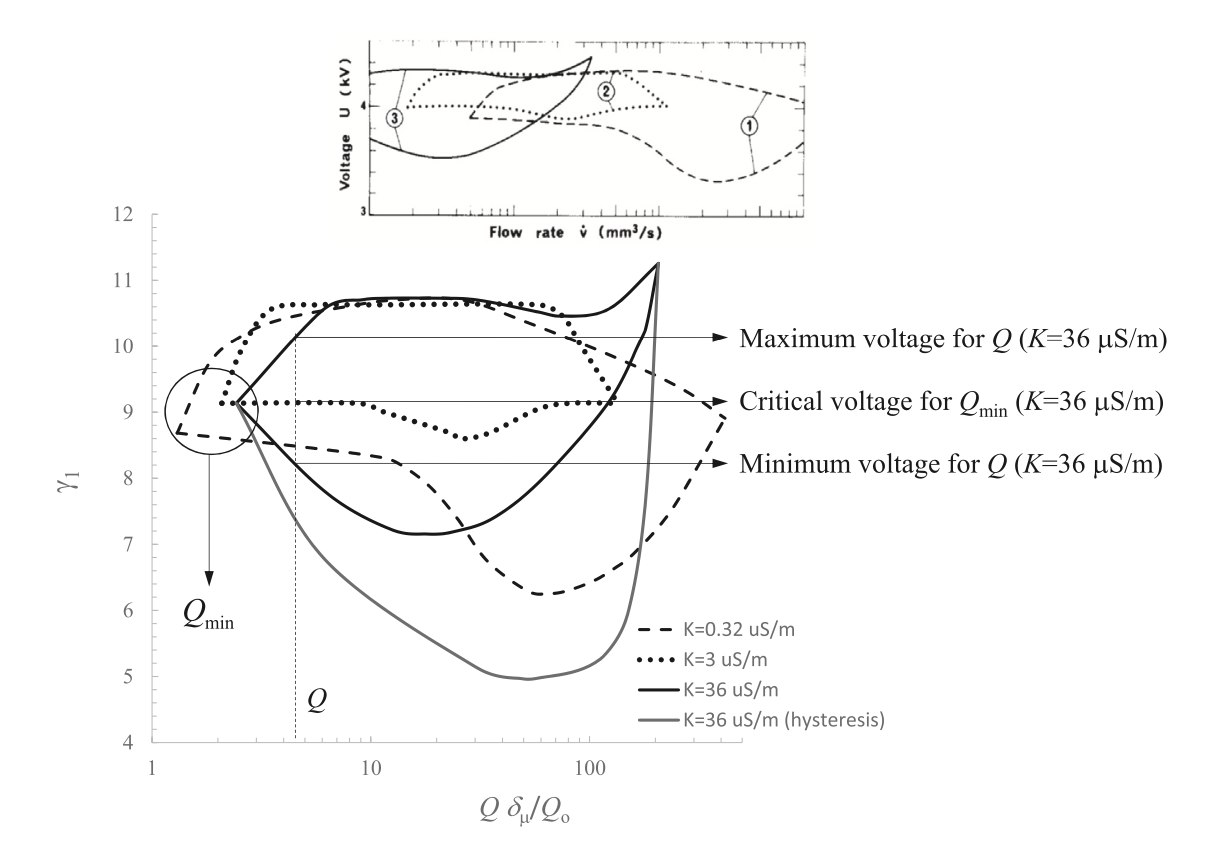
\includegraphics[width=13cm]{Figuras/ganan_calvo_map.png}
        \caption{Domains of existence (stability) of Taylor Cone Jets. \cite{gananCalvo} . The window formed by these points is where the system operated in the stable cone-jet. Operational windows depend of the liquid and configuration setup. Different windows are represented for different liquid conductivity. The X and Y axis are non-dimensional representation of electric potential and liquid flow rate, respectively.}
        \label{fig:ganan_calvo_fig}
    \end{figure}


    \begin{algorithm}
        \caption{MAP sequence in controller thread}\label{alg:mapping_algorithm}
        \begin{algorithmic}
        \Procedure{MAP}{$flowrate\_values$} 
            \ForAll{flowrate\_values}  \Comment{scanning in the flowrate range}
                \State \Call{send\_flowrate\_command}{flowrate}
                \State $voltage \gets voltage\_start$
                \While{$voltage \leq voltage\_stop$} \Comment{scanning in the voltage range}
                    \State \Call{send\_voltage\_command}{voltage}
                    \State \Call{sleep}{step \_time}
                    \State $voltage \gets voltage + step\_size$
                \EndWhile
            \EndFor
        \EndProcedure

        \end{algorithmic}
    \end{algorithm}

    In Figure \ref{fig:map2Data_fig} we can see the data acquired in this mapping experiments. The liquid used is pure ethanol. 
    Note that the experiment is composed of loops that increase voltage, change flowrate and repeat.


    \begin{figure}[H]
        \center
        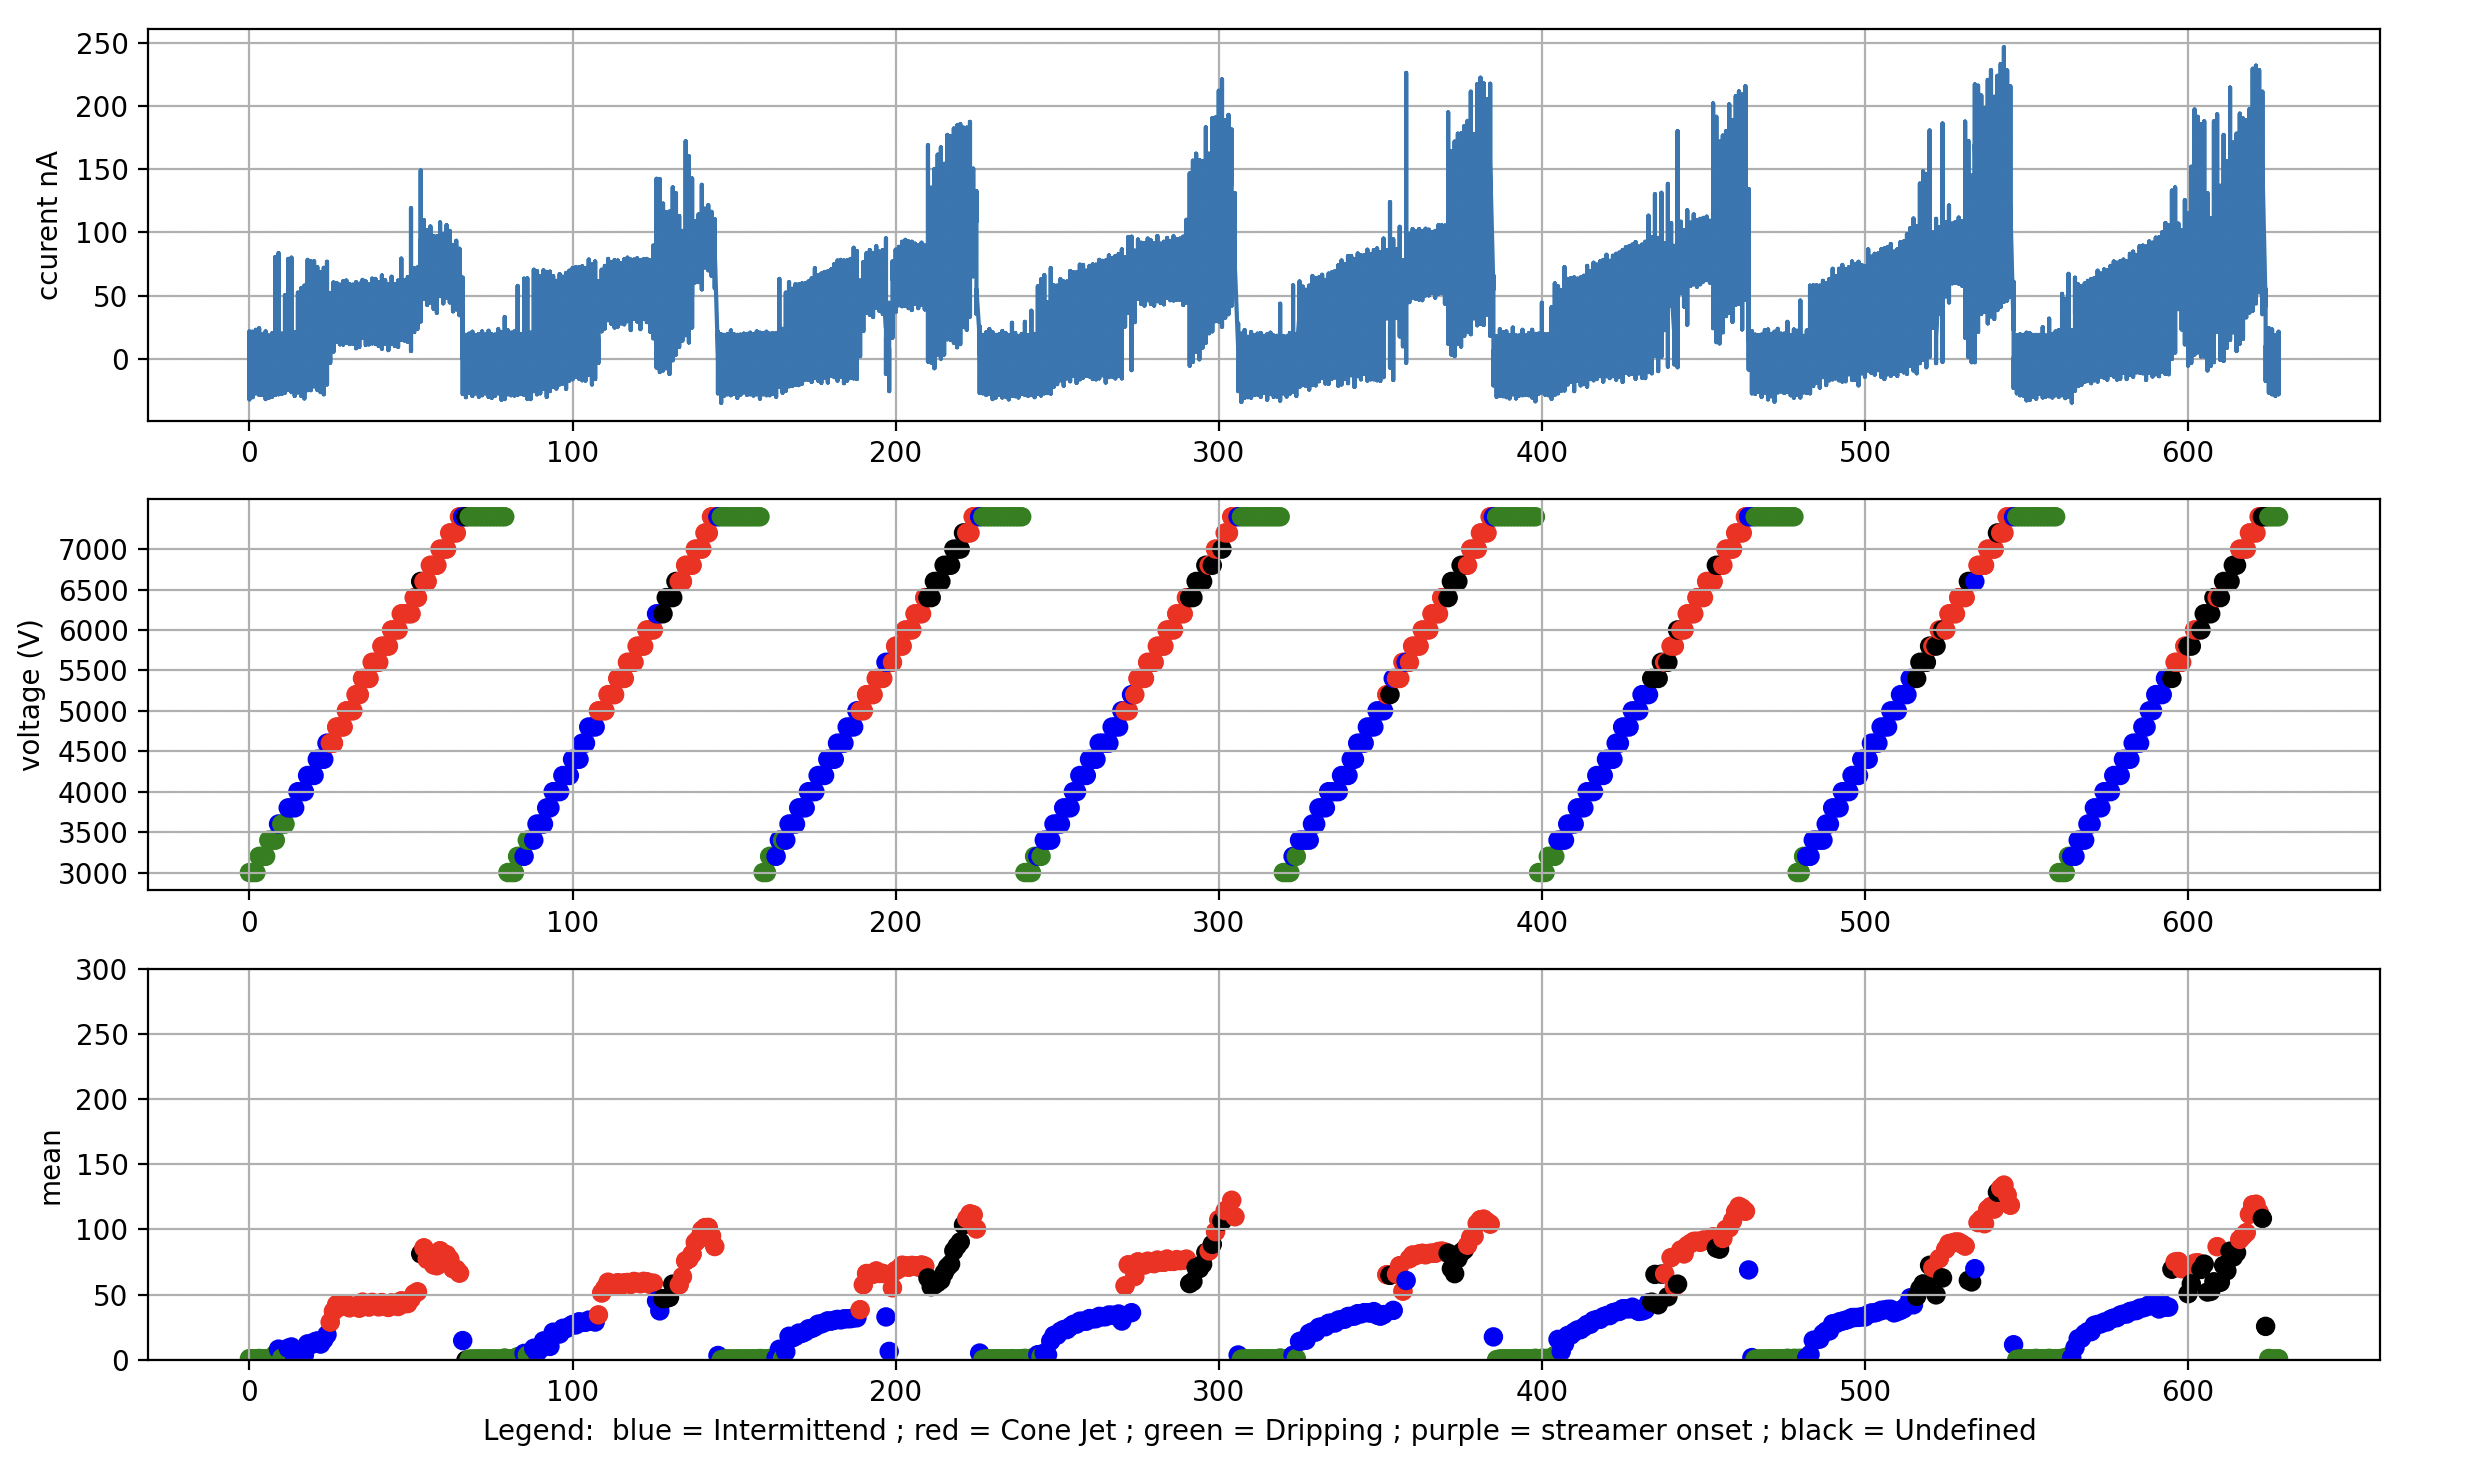
\includegraphics[width=15cm]{Figuras/report2/map2Data.png}
        \caption{Mapping Experiment data collected. The figure has 3 graphs with shared x axis representing the samples collected. The first is the current values collected through all the experiment.
        The second is the voltage values applied in each window of data collected. The colors represent the spraying classification defined by our routine.
        The third graph shows the current mean value of each data sample.}
        \label{fig:map2Data_fig}
    \end{figure}

    With all the data collected, classified and saved in real time, we can do further analysis and studies. For example, Figure \ref{fig:map3Data_fig} illustrate the data classified by our algorithm and displayed in a Voltage X FlowRate range of spraying modes with a specific liquid setup so that we can compare the automatic results with previous researchs, such as showed in figure \ref{fig:ganan_calvo_fig} and validate the algorithm.

    \begin{figure}[H]
        \center
        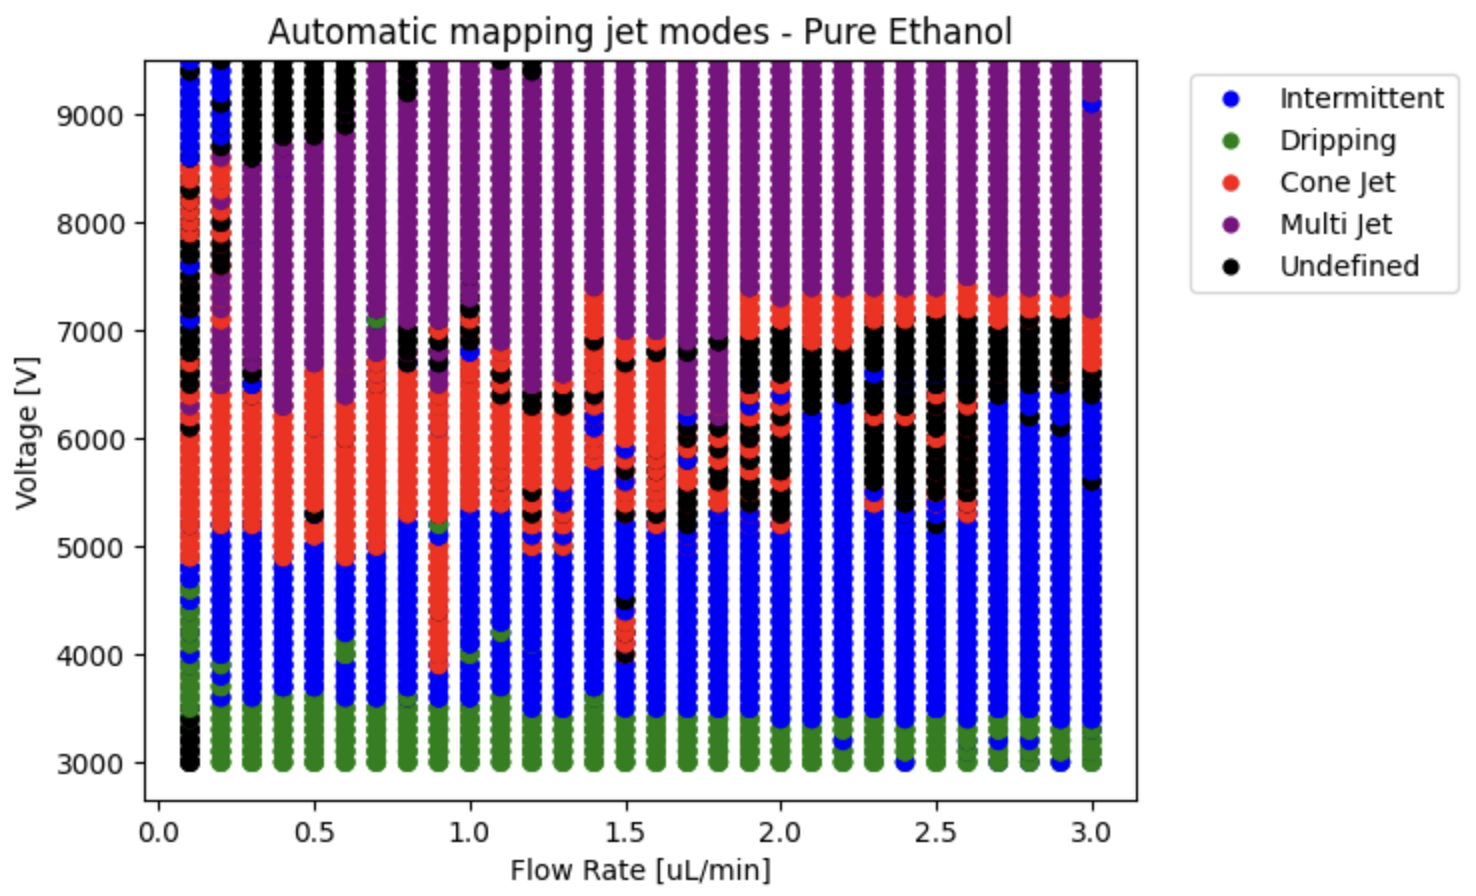
\includegraphics[width=15cm]{Figuras/report4/map-2023-03-02.png}
        \caption{Mapping Experiment for pure ethanol in ambient conditions with our capilary setup. The map shows the stability region of each electrospraying mode in the voltage and flowrate range.}
        \label{fig:map3Data_fig}
    \end{figure}



\subsection{Control}

    The control sequence is the only from our list of sequences that actually uses the feedback value. 
    As it is a closed loop control system the controller must be able to stabilize the system in the desired conditions.



\section{System Portability}
\label{sec:portability}

    Raspberry Pi


\clearpage